\section{Derivation of the compositional Feynman--Kac identity}\label{app:flow}
For a smooth positive factor density satisfying the Ornstein--Uhlenbeck forward equation,
\[
 \partial_u\log q_g=\tfrac12\nabla\cdot r_g-\tfrac12x^{\mathsf T}r_g+\tfrac12\|r_g\|^2.
\]
The prior $\varphi$ is stationary. Consequently, with $Q=\sum_g\|r_g\|^2$,
\[
 -\partial_u\log\rho=-\tfrac12\nabla\cdot R+\tfrac12x^{\mathsf T}R-\tfrac12Q.
\]
Put $S=\nabla\log\rho=-x+R$. Since $b_\kappa=R/2+\kappa S/2$,
\begin{align*}
 \rho^{-1}\left[-\nabla\cdot(b_\kappa\rho)+\tfrac\kappa2\Delta\rho\right]
 &=-\nabla\cdot b_\kappa-b_\kappa^{\mathsf T}S
 +\tfrac\kappa2(\nabla\cdot S+\|S\|^2)\\
 &=-\tfrac12\nabla\cdot R+\tfrac12x^{\mathsf T}R-\tfrac12\|R\|^2.
\end{align*}
Adding $g=(\|R\|^2-Q)/2$ yields \eqref{eq:fk}. Normalization subtracts $\E_{\rho/\int\rho}g$ from the potential. This calculation identifies the continuous path; existence of the normalized stochastic representation requires the corresponding integrability assumptions.

\section{Gaussian tail envelopes under an Euler transition}\label{app:envelope}
We give the full scalar argument used by Theorem~\ref{thm:tail}. Suppose
\[
 -\frac{x^2}{2V}-L|x|-C\le\log p(x)\le-\frac{x^2}{2V}+L|x|+C,
\]
and $g(x)=cx^2+r(x)$ with $|r(x)|\le L_g(1+|x|)$. Then
\[
 -\frac{D}{2V}x^2-(L+hL_g)|x|-C'
 \le\log[p(x)e^{hg(x)}]\le
 -\frac{D}{2V}x^2+(L+hL_g)|x|+C',\quad D=1-2hcV.
\]
For $D>0$, the integral is positive and finite, and its normalization has the same quadratic envelope with $V_t=V/D$. For $D<0$, the lower bound has a positive quadratic exponent and the integral diverges. At $D=0$, the remaining terms can give either behavior, so the general statement excludes equality.

Now suppose the propagated state is
\[
 Y=AX+q(X)+\tau\xi,\qquad |q(x)|\le K,\qquad \tau^2=\kappa h>0,
\]
where $X$ has the tilted density and $\xi\sim\Normal(0,1)$ is independent. For $z=y-Ax$, the Gaussian transition-density ratio satisfies
\[
 e^{-K|z|/\tau^2-K^2/(2\tau^2)}
 \le\frac{\varphi_\tau(z-q(x))}{\varphi_\tau(z)}
 \le e^{K|z|/\tau^2}.
\]
Use the reference joint density $\varphi_{\sqrt{V_t}}(x)\varphi_\tau(y-Ax)$. Its $Y$ marginal is Gaussian with variance $W=A^2V_t+\tau^2$, and its conditional distribution is
\[
 X\mid Y=y\sim\Normal\!\left(\frac{AV_t}{W}y,\frac{V_t\tau^2}{W}\right).
\]
Multiplying the density-ratio bounds by the envelope for the tilted input reduces the output bounds to conditional expectations of $\exp\{\pm(L_1|X|+L_2|y-AX|)\}$. For fixed $L_1,L_2\ge0$, Gaussian exponential moments and the triangle inequality give an upper bound $e^{C_1|y|+C_2}$. Jensen's inequality gives the lower bound
\[
 \E[e^{-L_1|X|-L_2|y-AX|}\mid Y=y]
 \ge e^{-L_1\E[|X|\mid Y=y]-L_2\E[|y-AX|\mid Y=y]}
 \ge e^{-C_3|y|-C_4}.
\]
It follows that $\log p_Y(y)=-y^2/(2W)+O(1+|y|)$. The argument also covers $A=0$ and bounded measurable $q$ without a monotonicity assumption. On a fixed finite grid with a fixed finite batch size, the finitely many factors, batches, and histories admit common finite residual and envelope constants up to each strictly positive step. Every such conditional normalizer is finite and positive. Repeating the argument along these histories proves Theorem~\ref{thm:tail}. For diagonal product models, a fixed index history leaves the coordinates conditionally independent, and the scalar argument applies coordinate by coordinate.

\section{A certificate for arbitrary affine controls}\label{app:general-control}
Suppose the true residual and its affine control have tail slopes $-a_g$ and $-t_g$, respectively. Set $e_g=a_g-t_g$, $T=\sum_g t_g$, and $c_0=(T^2-\sum_gt_g^2)/2$. The control-variate formula \eqref{eq:tail-estimator} remains conditionally unbiased when its residual is unbounded. For the empirical batch distribution $p$ on the $G$ factors, let $m=\sum_gp_ge_g$ and $s^2=\sum_gp_g(e_g-m)^2$. Its quadratic coefficients are
\begin{align}
 \widehat A(p)&=T+Gm,\\
 \widehat c(p)&=c_0+GTm-G\sum_gp_gt_ge_g+\tfrac12G(G-1)m^2
 -\tfrac12\left(\frac{G^2}{M-1}+G\right)s^2.\label{eq:controlled-c}
\end{align}
This identity follows by collecting the quadratic terms in \eqref{eq:tail-estimator}; the bounded parts of mixture scores contribute only $O(1+|x|)$ to the potential.

\begin{proposition}[Constant-batch certificate]\label{prop:control}
For Gaussian factors with arbitrary affine controls, the exact largest reachable variance is obtained by applying \eqref{eq:variance} to the $G$ constant batches at each step and retaining the largest value. The corresponding integrability decision is independent of every finite $M\ge2$. For equal-component-variance Gaussian mixture factors, the same recursion is exact for strict positive and strict negative denominator decisions under the tail-envelope assumptions of Theorem~\ref{thm:tail}.
\end{proposition}
\begin{proof}
Delete the nonpositive variance term from \eqref{eq:controlled-c}, obtaining $\widetilde c(p)$. This upper bound is convex on the probability simplex: its only quadratic term is the positive multiple $G(G-1)m^2/2$ of a squared affine function. Therefore $\widetilde c(p)\le\max_g\widetilde c(\delta_g)$, and all vertex values are attained by constant batches. If a denominator fails at the largest reachable variance, it fails at a vertex.

On the common positive-denominator domain, replacing $\widehat c$ by $\widetilde c$ increases the next variance. Write
\[
 n(p)=\sqrt V[1-h((1+\kappa)(T+Gm)+\kappa)/2],\qquad
 d(p)=1-2hV\widetilde c(p).
\]
Here $n$ is affine and $d$ is positive and concave. The quadratic perspective
\[
 n(p)^2/d(p)=\sup_{z\in\R}\{2zn(p)-z^2d(p)\}
\]
is convex in $p$, so its maximum on the simplex is attained at a vertex. The upper bound is exact there because $s^2=0$. Monotonicity in $V$ and induction complete the Gaussian proof. The mixture extension follows from Appendix~\ref{app:envelope}, since every fixed batch still has an affine drift plus a bounded term and a quadratic potential plus a linearly bounded term.
\end{proof}

For the constant batch containing factor $g$, the coefficients used by the implementation are
\[
 A_g^*=T+Ge_g,\qquad c_g^*=c_0+G(T-t_g)e_g+\tfrac12G(G-1)e_g^2.
\]
The check requires $G$ candidates per step and has no combinatorial dependence on $M$. For exact tail slopes $t_g=a_g$, every $e_g=0$, and all candidates coincide with the full-factor coefficients. With zero control, the simplex reduces to the scalar mean interval used in Theorem~\ref{thm:extreme}.

\begin{corollary}[Paired correction preserves the strict certificate]\label{cor:paired}
Under the strict-domain conditions of Proposition~\ref{prop:control}, averaging two independent batch drifts and using the paired weight from Appendix~\ref{app:local} gives the same strict integrability decisions as the unpaired estimator. The statement also applies to the raw unbiased estimator.
\end{corollary}
\begin{proof}
The negative squared-difference correction can only reduce the weight. Omitting it gives quadratic potential coefficient $\bar c=(c_1+c_2)/2$ and drift coefficient $\bar A=(A_1+A_2)/2$. The variance expression
\[
 (A,c)\longmapsto\frac{V[1-h((1+\kappa)A+\kappa)/2]^2}{1-2hVc}+\kappa h
\]
is jointly convex in $(A,c)$ on its positive-denominator domain, by the same quadratic-perspective identity. It is therefore at most the larger of the two unpaired next variances. Gaussian upper envelopes propagate under the omitted-correction transition; the actual positive weight obeys that upper bound after division by a finite positive normalizer. This proves finiteness along every paired history when the unpaired certificate stays strictly positive.

Conversely, take the maximizing constant batch at each step and use that same batch for both copies. This paired history has positive probability, the correction vanishes identically, and its tail variance follows the unpaired maximizing recursion. A strictly negative denominator therefore gives an infinite conditional integral. Tonelli's theorem gives divergence of the full paired operator. Gaussian factors also allow the exact equality decision; the mixture result leaves equality unclassified.
\end{proof}

\section{Second-order terms and paired weighting}\label{app:local}
This section records a local expansion to clarify the paired-correction ablation. Assume sufficient smoothness and integrable domination to justify expansion and normalization through third order for $h$ in a neighborhood of zero. A bounded-state setup with bounded smooth coefficients is one sufficient setting. These assumptions must be checked before applying the expansion; it cannot justify a kernel with an infinite normalizer.

At a fixed time, suppose $\E_B\widehat b=b$ and $\E_B\widehat g=g$. Define $C_b(x)=\Cov_B(\widehat b(x))$, $c_{bg}(x)=\Cov_B(\widehat b(x),\widehat g(x))$ and $v_g(x)=\Var_B(\widehat g(x))$. Let $Q$ denote the random kernel and $Q^0$ the full-coefficient Euler kernel. Expansion of the unnormalized kernel yields
\[
 (Q-Q^0)f=h^2\left\{\tfrac12 C_b:\nabla^2 f+c_{bg}^{\mathsf T}\nabla f+\tfrac12v_g f\right\}+O(h^3).
\]
The diffusion-dependent terms are common to both kernels. Expanding the ratio in \eqref{eq:kernel}, the normalized population difference is
\begin{equation}\label{eq:local-bias}
 \Phi(\eta)(f)-\Phi^0(\eta)(f)
 =h^2\left\{\tfrac12\eta(C_b:\nabla^2f)+\eta(c_{bg}^{\mathsf T}\nabla f)
 +\tfrac12\Cov_\eta(f,v_g)\right\}+O(h^3).
\end{equation}
The last term uses the covariance over the input population. A pointwise normalized kernel would be a different object. In particular, conditional score error alone does not specify this bias: its coupling with the potential enters through $c_{bg}$.

For two independent copies, use $\bar b=(\widehat b_1+\widehat b_2)/2$ and weight
\[
 \exp\left\{\tfrac h2(\widehat g_1+\widehat g_2)
 -\tfrac{h^2}{8}(\widehat g_1-\widehat g_2)^2\right\}.
\]
The expected squared difference is $2v_g$, cancelling the second-order potential-variance term. The remaining coefficient is
\[
 \tfrac14\eta(C_b:\nabla^2f)+\tfrac12\eta(c_{bg}^{\mathsf T}\nabla f).
\]
Thus paired weighting does not remove all second-order effects. For Gaussian factors, the event that both batches equal the same extreme batch at every step has positive probability; the correction vanishes on that history. Whenever Theorem~\ref{thm:extreme} gives a divergent extreme history, this paired version also has an infinite normalizer.

\section{Without-replacement comparison}\label{app:without-replacement}
The with-replacement assumption is substantive. For a uniformly sampled subset of size $2\le M\le G$, an unbiased potential estimator is
\[
 \widehat g_{\mathrm{WOR}}=\frac{G(G-1)}{M(M-1)}\sum_{i<j}r_{I_i}^{\mathsf T}r_{I_j}.
\]
Distinct indices are sampled, so its pair coefficient differs from \eqref{eq:U}. For the same one-step example \eqref{eq:counterexample}, exact subset enumeration gives the following maximum quadratic coefficients and minimum denominators:
\[
\begin{array}{c|ccc}
 M & 2 & 3 & 4\\ \hline
 \max\widehat c_{\mathrm{WOR}} & 2 & 29/33 & 346/693\\
 \min D & 47/355 & 659/1065 & 2503/3195
\end{array}
\]
All three without-replacement one-step operators are finite. At $M=G$ the estimator equals the full-factor potential. This analytic comparison shows that the failure established for every finite with-replacement $M$ does not transfer to an arbitrary subsampling scheme. It does not assert multi-step stability of without-replacement updates for other grids or factor sets.

\section{Complete benchmark certificate}\label{app:full-results}
Every executed benchmark configuration is classified in Figure~\ref{fig:complete-certificate}. The coordinate-wise tests classify the population operator before inspecting any particle outcome.
\begin{figure}[ht]
 \centering
 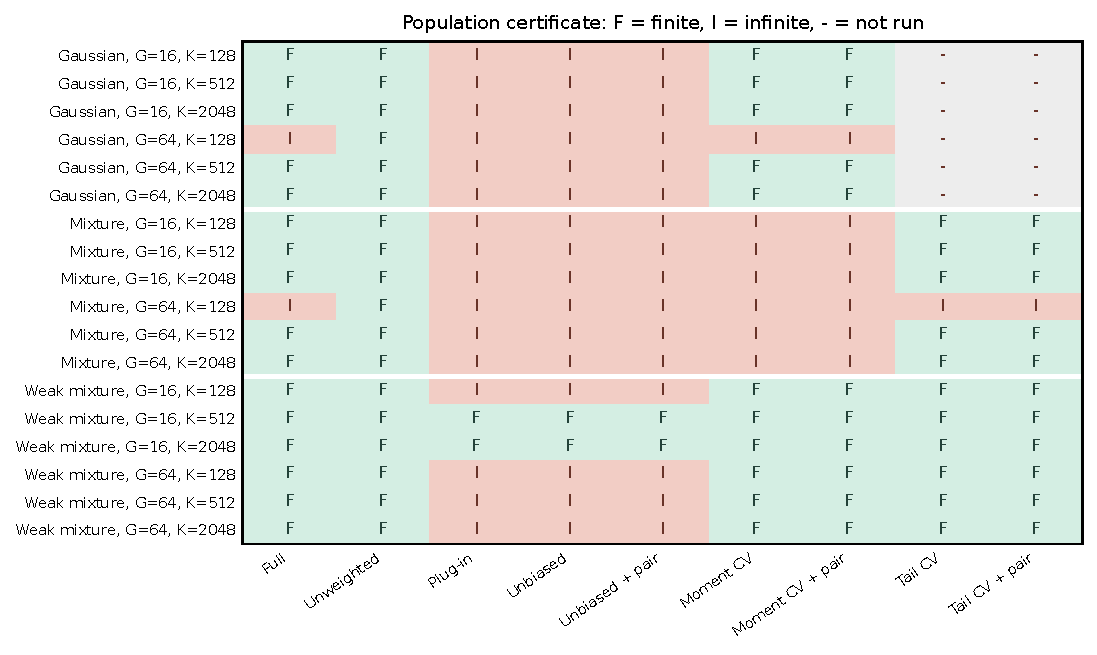
\includegraphics[width=\linewidth]{figures/integrability_grid.pdf}
 \caption{Complete certificate for the executed benchmark methods. The statuses agree for $d=1$ and $d=8$, so the dimensions share a row. Each row therefore represents ten executed cells per method across both dimensions and five seeds. The classification is derived from the population recursion, independently of particle outcomes.}
 \label{fig:complete-certificate}
\end{figure}

\section{Factor families and implementation details}\label{app:protocol}
For indices $g=0,\ldots,G-1$ and $j=0,\ldots,d-1$, set $\theta_{gj}=2\pi(g+0.37j)/G$. Each factor is a product over coordinates. The Gaussian family uses variance $v_{gj}=0.5+0.15\sin\theta_{gj}$ and mean $0.35+0.3\cos\theta_{gj}$. The two-component mixture family uses the same component variance, component means
\[
 0.1\cos\theta_{gj}\ \pm\ (0.7+0.2\cos(2\theta_{gj})),
\]
and positive-component weight $0.5+0.1\sin(\theta_{gj}+0.7)$. The weak mixture family uses
\[
 v_{gj}=\left[1+\frac{4+2\sin\theta_{gj}}G\right]^{-1},\qquad
 \mu_{gj,\pm}=\frac{0.4\cos\theta_{gj}}G
 \pm\frac{0.6+0.1\cos\theta_{gj}}{\sqrt G},
\]
with the same component weights. All component variances are below one, so their residual tail precisions are nonnegative. The Gaussian and ordinary mixture have identical tail certificates despite their different interior geometry.

At each step, weights are multiplied using the left-endpoint potential and states receive the Euler drift and Gaussian noise. Systematic resampling is performed when the effective sample size is below half the particle count. Computation uses double precision, one GPU per task, four allocated CPU cores, and one numerical-library thread. Timing includes sampling, weighting, and resampling, with GPU synchronization at the measured boundaries. Factor reference quadrature and final metric computation are outside the sampler timing. The score-evaluation count records particle--factor evaluations and counts both batches in paired methods.

The raw endpoint sample for each benchmark cell contains all particles and normalized weights. Reference grids, densities, cumulative distribution functions, step metrics, runtime metadata, configuration, and completion records accompany each cell. The one-step study retains weighted histograms and the largest-weight particles, as specified before execution. Independent verification recomputes benchmark metrics using separate SciPy routines and checks all recovered file hashes against the remote manifest.
